\documentclass[conference,10pt]{IEEEtran}

\usepackage{cite}
\usepackage{amsmath,amssymb,amsfonts}
\usepackage{algorithmic}
\usepackage{graphicx}
\usepackage{textcomp}
\usepackage{xcolor}
\usepackage{booktabs}
\usepackage{tabularx}
\usepackage{array}
\usepackage{url}
\usepackage{hyperref}

\hypersetup{
    colorlinks=true,
    linkcolor=blue,
    citecolor=blue,
    urlcolor=blue,
    bookmarks=true,
    bookmarksnumbered=true,
    pdftitle={A Flexible Offline Mobile Payment Architecture Using NFC and HCE: A Cost-Optimized Approach for Low-Infrastructure Environments},
    pdfauthor={Nabil Al-Mekhlafi, Ahmed Al-Mutawakel},
    pdfsubject={Mobile Payment, NFC, HCE, Mobile Data Routing},
    pdfkeywords={Offline Mobile Payment, SoftPOS, NFC, HCE, Android SDK, Mobile Data, Cost Model, Financial Inclusion}
}

\begin{document}

\title{A Flexible Offline Mobile Payment Architecture Using NFC and Host Card Emulation: A Cost-Optimized Approach for Low-Infrastructure Environments}

\author{
\IEEEauthorblockN{Nabil Al-Mekhlafi}
\IEEEauthorblockA{\textit{Faculty of Computer Science} \\
\textit{Sana'a University}\\
Sana'a, Yemen \\
nabil.almekhlafi@su.edu.ye}
\and
\IEEEauthorblockN{Ahmed Al-Mutawakel}
\IEEEauthorblockA{\textit{Faculty of Computer Science} \\
\textit{Sana'a University}\\
Sana'a, Yemen \\
a.almutawakel@su.edu.ye}
}

\maketitle

\begin{abstract}
Mobile payment systems in low-infrastructure regions remain constrained by intermittent internet connectivity and prohibitive hardware costs. In Yemen, for instance, only 17.7\% of the population has internet access, and existing wallet services (Alkuraimi, Jawali, Jaib, MFloos) require a constant connection to the cloud, forcing merchants and customers to revert to cash during outages. We present ``Atheer,'' an offline-first payment architecture that combines a four-layer backend, an Android SDK with Host Card Emulation (HCE), Limited Use Keys (LUKs), and a novel Mobile Data Routing model with Partner-Subsidized Billing. Unlike prior approaches relying on a private APN, Atheer routes settlement traffic over standard mobile data with a tightly optimized 180-byte payload, while the partner wallet absorbs the merchant's data cost via a B2B contract. A Discrete Event Simulation across six load levels (5--500 TPS, $N=10$) shows that the mobile-data path sustains a 97.6\% success rate at 500 TPS with P95 latency of 672 ms, while the public-internet baseline collapses to 76.2\%. The cost model demonstrates that data expenditure remains below 0.5\% of the partner wallet's Merchant Discount Rate revenue, making the architecture economically sustainable for nationwide rollout in fragile economies.
\end{abstract}

\begin{IEEEkeywords}
Offline Mobile Payment, SoftPOS, NFC, Host Card Emulation (HCE), Android SDK, Mobile Data Routing, Partner-Subsidized Billing, Payload Optimization, Financial Inclusion.
\end{IEEEkeywords}

% =================================================================
\section{Introduction}
% =================================================================

The rapid adoption of smartphones and Near Field Communication (NFC) technology has accelerated the development of cashless economies. However, this development has been distributed unequally across regions. With a national internet penetration of 17.7\% \cite{datareportal2024}, Yemen's physical network infrastructure has suffered years of deferred maintenance, resulting in chronic outages, high latency, and low bandwidth \cite{ookla2024}. Cloud computing has gained traction in Yemeni institutions \cite{alhashedi2024, almekhlafi2018}, but modern payment systems require real-time transaction authorization through active cloud systems, which is rarely feasible in this context \cite{isoc2024}.

Yemeni customers do have access to mobile wallet systems provided by early financial inclusion pioneers such as Alkuraimi, Jawali, Jaib, and MFloos. However, these legacy systems rely on SMS or USSD as fallback channels when connectivity is compromised. These channels are slow and do not provide end-to-end encryption, which greatly diminishes the user experience \cite{gsma2023}. Hence, when the network goes down, merchants and customers have no other option than to revert to cash.

To address these limitations, we built ``Atheer,'' a proprietary Android SDK and backend gateway with a four-layer backend architecture. The client-side SDK preloads several batches of cryptographic tokens (Limited Use Keys) and uses NFC, in combination with Host Card Emulation, to complete transactions without requiring the customer device to maintain an active internet connection. The merchant device then submits the signed payload via standard mobile data to the Atheer Gateway Switch for verification and ledger update.

Three contributions distinguish Atheer from prior work:

\begin{itemize}
\item A dual-component structure (edge SDK + gateway switch) with a four-layer architecture integrating Mobile Data Routing with Partner-Subsidized Billing, multi-provider gateway verification, and Zero-CapEx SoftPOS.
\item A Pre-Authorized Biometric Cryptogram that temporally binds the signing key to the Trusted Execution Environment (TEE) via a biometric constraint and a 60-second temporal window, combined with server-side Zero-Trust verification.
\item A formal cost model proving that a tightly optimized 180-byte payload allows the partner wallet to absorb the merchant's mobile data cost while keeping data expenditure below 0.5\% of Merchant Discount Rate (MDR) revenue, validated by a Discrete Event Simulation across six load levels (5--500 TPS) showing 97.6\% success at peak load.
\end{itemize}

% =================================================================
\section{Related Work}
% =================================================================

Increased research interest has been drawn to financial networks that operate offline. For the International Monetary Fund (IMF), offline functionality is a prerequisite for financial inclusion in developing economies \cite{imf2022}. Similarly, the World Bank has invested in Yemen's digital infrastructure development \cite{worldbank2023}. However, the majority of local deployments overlook essential cryptographic and architectural frictions, limiting their ability to scale.

\subsection{Legacy Channels: USSD and SMS-Based Systems}

The current user base of SMS and USSD-based solutions remains the largest in Yemen. Wallets such as Alkuraimi and Jaib benefit from this user base because their services do not require an active internet connection. However, this comes at a significant tradeoff. According to the GSM Association, these communication methods exhibit substantial cryptographic weaknesses, including the absence of end-to-end encryption, exposing messages to man-in-the-middle attacks and eavesdropping \cite{gsma2023}. Asynchronous SMS routing for retail payments is now functionally obsolete.

\subsection{Hardware-Based NFC Architectures}

Recent localized efforts have introduced circuitry-based NFC systems, often branded as the ``Mobile Money'' initiative. These are considered hardware-based because merchants must purchase proprietary Point-of-Sale (POS) terminals \cite{brandpos2024}. This capital expenditure (CapEx) barrier, combined with the fact that these terminals still rely on cloud connectivity for balance verification, creates a single point of failure in regions where network outages are frequent \cite{isoc2024}.

\subsection{SoftPOS and HCE as Contemporary Constructs}

A growing trend in global payments research focuses on software-oriented models \cite{kemper2022}. Ahamad \cite{ahamad2022} created a hybrid NFC system tailored for closed enterprise communities; while it reduced internet reliance, it lacked the scalability needed for national deployment. Oladapo et al. \cite{oladapo2024} demonstrated that Host Card Emulation (HCE) combined with Limited Use Key tokenization (a model referred to as SoftPOS) transforms standard mobile devices into flexible acceptance terminals while addressing replay attacks. Gbadebo \cite{gbadebo2024} developed Short-Lived Distributed Ledger Technology (SLDLT) that supports multiple transport mechanisms (NFC, Bluetooth, SMS) for offline transaction closure. The ``Kipaad'' model from Iran, which uses SIM-embedded components, fits high-volume micro-transport transactions but does not generalize to multi-provider retail payments. Macroeconomic indicators suggest contactless payments will grow exponentially through 2028 \cite{juniper2024}, provided existing infrastructural constraints are addressed.

\subsection{Identified Research Gap}

The combined insights from the literature suggest that achieving resilience in offline payment systems requires a layered, redundant approach that includes local authorization, hardware-independent (zero capital expenditure) deployment, and multi-provider interoperability. While individual studies report success in Nigeria, Iran, and Ghana, none combine client-side internet independence, zero-CapEx SoftPOS, and a cost-optimized mobile-data routing model into a single approach. This is the gap that Atheer addresses. We pair an HCE-based edge layer with deterministic switching and a payload-optimized mobile-data pathway designed for challenging connectivity conditions, while keeping the model economically sustainable via partner-subsidized billing.

% =================================================================
\section{Methodology}
% =================================================================

We employed the Design Science Research (DSR) methodology \cite{hevner2004, peffers2007}, a systematic approach to developing and evaluating IT artifacts that address real-world problems. Using DSR, we designed, built, and evaluated Atheer, a multi-layered architecture for offline-first mobile payments employing offline tokenization, NFC, HCE, and mobile-data routing with partner-subsidized billing. Table~\ref{tab:dsr} maps DSR phases to the corresponding activities in this work.

\subsection{Ethical Considerations}

In line with the DSR principles and to address legitimate ethical concerns raised in prior peer review, this study does not evaluate or assess the security of any named financial institution in Yemen. References to wallets such as Alkuraimi, Jawali, Jaib, and MFloos appear only in the context of market description; no claims about their cryptographic posture are made. The simulation is fully synthetic, does not use any real banking data, and does not require permission from any operator. All cost assumptions are derived from publicly available pricing references (ITU, GSMA, Cable.co.uk).

\subsection{Simulation-Based Evaluation (DES)}

Since live testing on real banking infrastructure in an active conflict zone is infeasible, we adopted Discrete Event Simulation (DES). The DES measures end-to-end tail latency (P95), success rates, and overhead incurred by the Atheer Switch under realistic operating conditions (latency, congestion, packet loss, and full loss of public connectivity). A theoretical security analysis was also performed to assess the architecture's resilience against replay, interception, and man-in-the-middle (MitM) attacks. The simulation source code is publicly available as a research artifact \cite{mutawakel2024}.

\begin{table*}[t]
\caption{DSR Phase Mapping with Atheer Research Project}
\label{tab:dsr}
\centering
\footnotesize
\begin{tabular}{@{}p{2.8cm}p{12cm}@{}}
\toprule
\textbf{DSR Phase} & \textbf{Activity in This Work} \\
\midrule
Problem Identification & Engagement with payment mechanisms on Yemen's payment infrastructure: internet reach, outage frequency, CapEx barriers, and cryptographic weakness of incumbent SMS/USSD channels (Sections~I--II). \\
Design \& Development & Engineering the four layers of Atheer: edge SDK, mobile-data network layer, gateway switch, integration layer (Sections~IV--V). \\
Demonstration & Tracing of system workflow across three operation phases (token provision, offline NFC exchange, mobile-data settlement) with architecture diagrams (Section~V). \\
Evaluation & Discrete-Event Simulation on six load levels (5--500 TPS, $N=10$), yielding P95 latency and success-rate metrics with 95\% confidence intervals (Section~VII). \\
Communication & This paper and the open-source simulation artifact \cite{mutawakel2024}. \\
\bottomrule
\end{tabular}
\end{table*}

% =================================================================
\section{Proposed Architecture}
% =================================================================

Avoiding one-size-fits-all models, we built Atheer using a distributed architecture with four distinct layers (Fig.~\ref{fig:arch}). The Edge Layer houses the merchant's SoftPOS app and the offline client SDK. The Network Layer handles routing over mobile data with a partner-subsidized billing model. The Switch Layer acts as an autonomous transaction gateway. The final Integration Layer interfaces with Hardware Security Modules (HSMs) and the main banking ledger.

\begin{figure}[t]
\centering
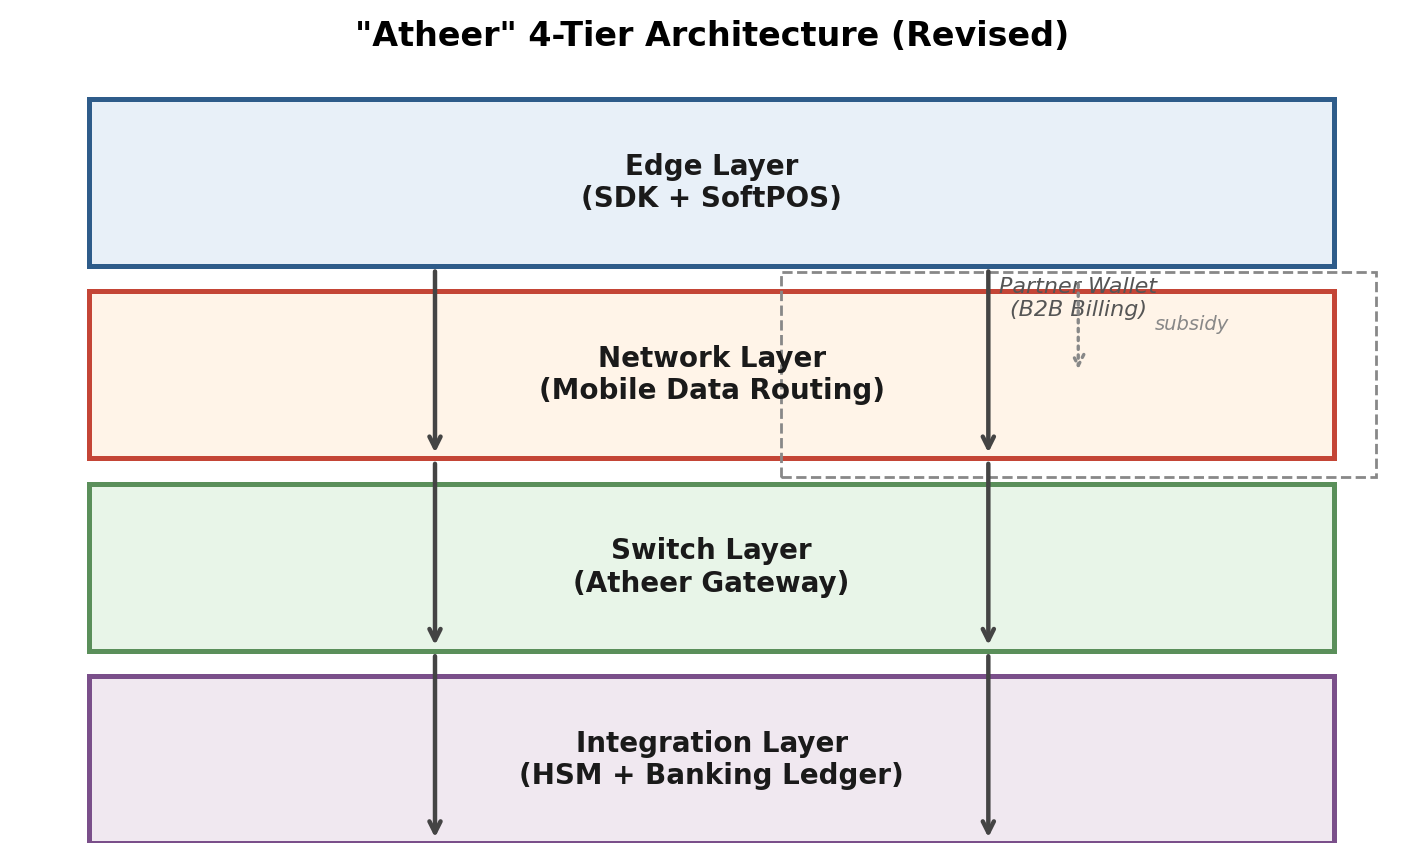
\includegraphics[width=\columnwidth]{fig1_architecture.png}
\caption{Revised four-tier architecture of Atheer. Financial data is routed over standard mobile data with a tightly optimized 180-byte payload, while the partner wallet subsidizes the merchant's data cost through a B2B contract.}
\label{fig:arch}
\end{figure}

\subsection{Edge Layer: The Embeddable Modular Library}

As shown in Fig.~\ref{fig:layered}(a), the client library is a lightweight Android module that integrates into existing wallet apps without restructuring their codebase. The system uses five components to carry out offline transactions:

\begin{enumerate}
\item \textbf{Cryptographic Key Manager:} Maintains two keys in the Trusted Execution Environment (TEE): a symmetric AES-256/GCM key for local data encryption and an asymmetric signing key pair. The private key is locked and inaccessible until biometric user authentication occurs.

\item \textbf{Secure Token Vault:} Primary Account Numbers (PANs) are never stored. Instead, Limited Use Keys (LUKs) are kept in an encrypted vault. When the application detects an Internet connection, it downloads batches of these tokens. Each token has a rigid lifecycle: Available $\rightarrow$ Allocated $\rightarrow$ Consumed.

\item \textbf{HCE Engine:} Operates on Android's native Host Card Emulation. When an NFC signal is detected from a merchant device, tokens are transmitted via an Application Protocol Data Unit (APDU), but only during an Armed Session: a 60-second window opened by successful biometric authentication.

\item \textbf{Network Routing Unit:} Monitors the connection state and decides whether to route settlement requests over mobile data (preferred) or queue them for deferred transmission if no data is available.

\item \textbf{Encrypted Local Data Store:} A TEE-managed key protects the local database, which records transactions and synchronization status (Unsynchronized vs. Synchronized) to ensure consistency when the device reconnects.
\end{enumerate}

\begin{figure}[t]
\centering
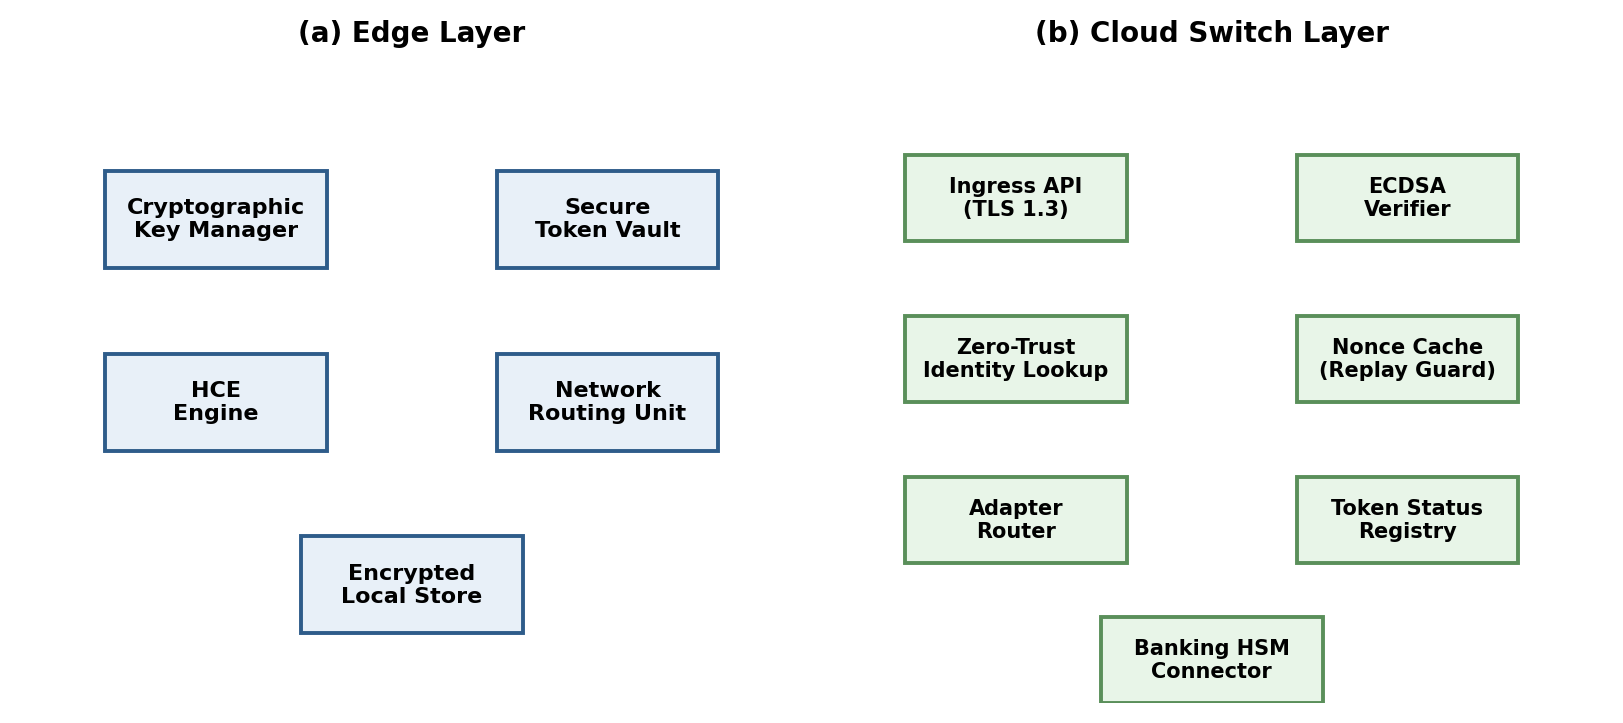
\includegraphics[width=\columnwidth]{fig2_layered.png}
\caption{Atheer layered system. (a) Edge layer modules. (b) Cloud Switch layer modules.}
\label{fig:layered}
\end{figure}

\subsection{Edge Layer: SoftPOS Implementation}

The software-based POS (SoftPOS) merchant module enables any NFC-capable smartphone to function as a POS terminal \cite{kemper2022, pci2023}, reducing capital expenditure considerably for micro enterprises.

\textbf{NFC Reader Integration:} A merchant application (in Active Reader Mode) manages NFC interaction with the client phone to receive the APDU packet containing an encrypted token \cite{dinh2021}.

\textbf{Transaction Encapsulation:} The SoftPOS terminal maintains a Zero-Knowledge environment and holds no decryption keys. Its function is to receive the encrypted token, payment amount, merchant ID, and Application Transaction Counter (ATC), wrap and digitally sign the payload, and forward it to the gateway.

\subsection{Network Layer: Mobile Data Routing with Partner-Subsidized Billing}

This layer replaces the original private-APN model with a more deployable approach. Instead of requiring a dedicated cellular tunnel (which depends on B2B agreements with mobile network operators that are difficult to obtain in fragile economies), Atheer routes settlement traffic over the merchant's standard mobile data connection. The key insight is that the resulting payload is so small that the cost becomes negligible, and a partner wallet can absorb it through a B2B contract.

\textbf{Payload Optimization:} The settlement packet is tightly compressed to 180 bytes by minimizing field lengths and removing redundant headers. Figure~\ref{fig:packet} shows the breakdown. The packet consists of: a 32-byte routing header (merchant ID, transaction ID), a 32-byte LUK token, a 4-byte ATC, an 8-byte amount field, a 16-byte nonce, an 8-byte timestamp, a 64-byte ECDSA signature (P-256), and a 28-byte AES-GCM IV plus authentication tag. After header compression (variable-length encoding of merchant ID and transaction ID), the effective size is reduced from 192 bytes to 180 bytes.

\begin{figure}[t]
\centering
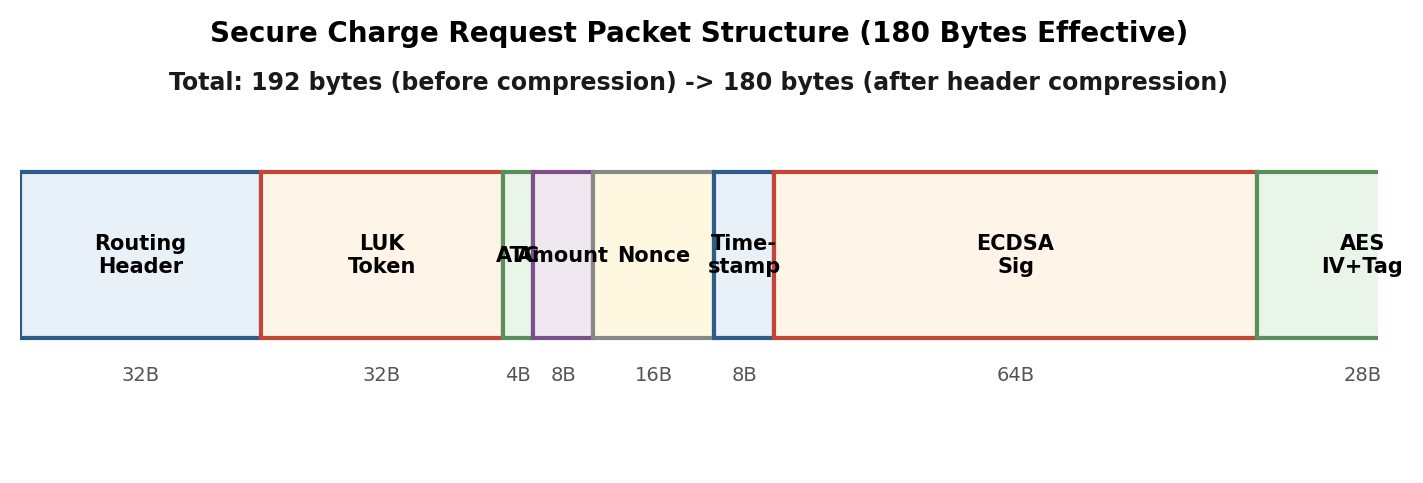
\includegraphics[width=\columnwidth]{fig5_packet.png}
\caption{Secure Charge Request packet structure. Total: 192 bytes uncompressed, 180 bytes effective after header compression.}
\label{fig:packet}
\end{figure}

\textbf{Partner-Subsidized Billing:} Under this model, the partner wallet signs a B2B agreement with the merchant's mobile network operator to reimburse data costs for traffic identified as Atheer settlement. The wallet identifies its traffic via a TLS 1.3 certificate pin and a designated SNI; the MNO accounts for these bytes separately and invoices the wallet monthly. Because the payload is only 180 bytes per transaction, the cost is dwarfed by the Merchant Discount Rate (MDR) revenue the wallet earns on each successful transaction. Section~\ref{sec:economic} formalizes this claim.

\textbf{Security Hardening:} Without network-layer isolation (as a private APN would provide), Atheer compensates through application-layer security: TLS 1.3 \cite{rfc8446} with certificate pinning, ECDSA signatures, and the 180-byte payload minimizing the surface for traffic analysis. DDoS protection is delegated to the gateway's edge, which implements rate limiting and a Web Application Firewall (WAF).

\subsection{Switch and Integration Layer: Multi-Provider Gateway}

The Atheer Gateway Switch is a lightweight intermediary that uses the Adapter Pattern to integrate the edge SDK with multiple banking backend systems. It hosts a Unified API Contract with two main functionalities:

\begin{itemize}
\item \textbf{Token Provisioning:} Devices call this endpoint when online to retrieve new token batches and register hardware-attested public keys.

\item \textbf{Payment Processing:} The switch retrieves signed merchant payloads and validates the asymmetric signature using the device's pre-registered public key.
\end{itemize}

A major design decision is the separation of validation from the actual financial transaction. As shown in Fig.~\ref{fig:layered}(b), upon receiving a payload at the Ingress API, the switch performs: (i) ECDSA asymmetric signature validation, (ii) Zero-Trust identity extraction (client verified only against the internal database), and (iii) in-memory nonce verification against replay attacks. After these checks, the adapter router transmits the transaction to the appropriate banking institution and updates the token status to Consumed.

% =================================================================
\section{System Workflow}
% =================================================================

Internet access in Yemen is severely limited, with about 82.3\% of the population lacking stable access \cite{datareportal2024}. Atheer's operational protocol is designed with these challenges in mind, employing an asynchronous hybrid model that segments transactions into three phases: online provisioning, fully offline NFC, and final settlement over mobile data with deterministic, risk-managed logic applied at the edge. Figure~\ref{fig:interaction} illustrates the interaction architecture.

\begin{figure}[t]
\centering
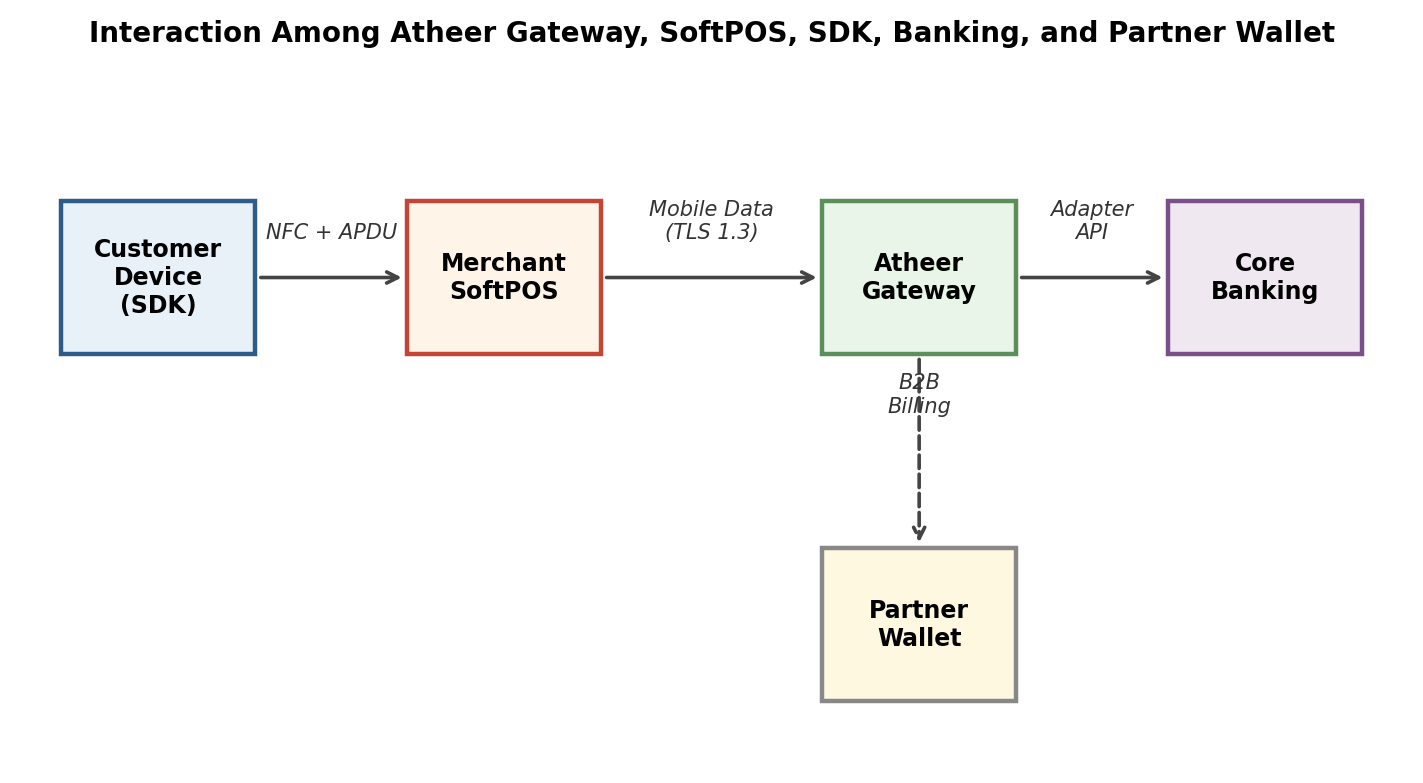
\includegraphics[width=\columnwidth]{fig3_interaction.png}
\caption{Interaction architecture among the Atheer Gateway, merchant SoftPOS, offline SDK, core banking system, and partner wallet.}
\label{fig:interaction}
\end{figure}

\subsection{Phase 1: Cryptographic Initialization and Token Provisioning}

This step requires the client's active internet connection (either Wi-Fi or mobile data) to download cryptographic material and ready the internal vault for offline activities. To address concerns about relying on the same public network that the architecture criticizes, Atheer supports two provisioning pathways:

\begin{enumerate}
\item \textbf{In-Band Provisioning over TLS 1.3:} The default pathway. The client establishes a TLS 1.3 channel with certificate pinning to the Atheer Gateway. Hardware attestation keys embedded in the TEE bind the device identity to the issued tokens. While this pathway does use the public internet, the security guarantees come from transport-layer encryption and hardware-anchored device identity, not from network-layer isolation.

\item \textbf{Out-of-Band Provisioning at Bank Branches:} For high-value merchants, tokens can be provisioned at a partner bank branch over a private LAN. This pathway is reserved for cases where the public internet is completely unavailable for extended periods.
\end{enumerate}

\subsection{Phase 2: Offline Execution and Pre-Authorized Biometric Cryptogram}

The SDK's role as a local decision-maker enables offline payment authorizations.

\textbf{Biometric Authentication and Session Arming:} Users authenticate at the TEE level. Upon success, the user may sign an Armed Session for 60 seconds. During this window, the library generates a signed payload that binds the token to that moment in time (Pre-Authorized Biometric Cryptogram).

\textbf{NFC Detection and HCE Activation:} The SoftPOS SDK triggers HCE to begin standard EMV contactless handshaking \cite{emvco2023} when an EM field is detected.

\textbf{Local Risk Checks:} Before transmission, the library checks: (i) token validity (is the token unspent in the local registry?) and (ii) session state (is the Armed Session still active?).

\textbf{Signed Payload Transmission:} After both checks pass, an APDU transaction is sent to the merchant device, ending the session and marking the token as Consumed. Figure~\ref{fig:state} presents the state diagram.

\begin{figure}[t]
\centering
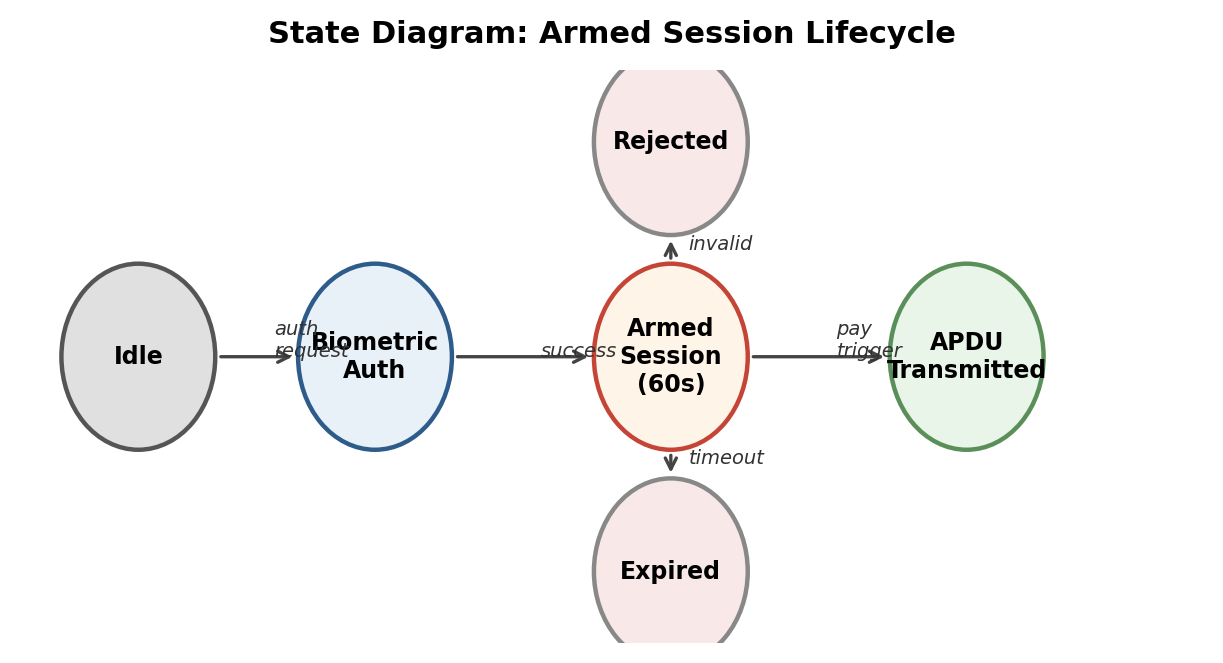
\includegraphics[width=\columnwidth]{fig4_state_diagram.png}
\caption{State diagram of an armed session.}
\label{fig:state}
\end{figure}

\subsection{Phase 3: Gateway Routing and Secure Settlement via Mobile Data}

Settlement relies on an internal path that uses the merchant's mobile data connection, secured by TLS 1.3 and the partner-subsidized billing model.

\textbf{Packet Encapsulation:} The SoftPOS device encapsulates the APDU packet within a Unified Charge Request Payload, consisting of an unencrypted public routing header, an AES-encrypted core payload, and the merchant's ECDSA digital signature.

\textbf{Mobile Data Routing:} The payload is transmitted over standard mobile data (LTE/3G) with TLS 1.3 and certificate pinning. Because the payload is only 180 bytes, it fits within a single TCP segment and completes within one round trip under most network conditions.

\textbf{Settlement and Token Neutralization:} The switch's Ingress API receives the payload, performs signature, identity, and nonce checks in memory (under 20 ms), and routes the verified transaction to the corresponding bank. Upon completion, the LUK State Registry marks the token as permanently Consumed and sends an acknowledgment back.

% =================================================================
\section{Security Analysis}
% =================================================================

Atheer integrates security across the storage, edge, and network routing stack. This section analyzes each security mechanism in detail.

\subsection{Confidentiality: Tokenization and AES-256 GCM}

At no point are static PANs stored or transmitted. All sensitive data is replaced by dynamic tokens.

\textbf{Data At Rest:} Tokens are stored in phone local memory encrypted with AES-256 GCM. The symmetric key resides in the Android Keystore (TEE enclave) and is inaccessible even on rooted devices.

\textbf{Data In Transit:} Each transaction is encrypted and encapsulated into a structured secure packet (Fig.~\ref{fig:packet}). The routing header remains unencrypted while the core payload is AES-encrypted. The merchant terminal sees only ciphertext, implementing strict Zero-Knowledge design.

\subsection{Integrity: Cryptographic and Biometric Security}

A pre-authorized biometric cryptogram prevents post-NFC handshake tampering. The local cryptographic engine signs the payload with a private key anchored in the TEE, accessible only during a 60-second armed session following biometric verification. The signature binds the token to a specific timestamp; any modification invalidates the signature. The Atheer Gateway validates the signature using the public key registered during provisioning, rejecting tampered transactions automatically.

\subsection{Replay Attacks}

The most severe threats to offline payment systems are synchronous and asynchronous replay attacks \cite{hancke2010}. Atheer uses dual-locking:

\textbf{Limited Use Keys (LUKs):} Each token is restricted to a single transaction. Once used, the token is set to Consumed in both the local SDK and the central switch registry, and this state cannot be reverted.

\textbf{Cryptographic Nonces:} Each payload includes a unique random nonce, checked against an in-memory cache at the switch. Duplicate nonces cause immediate packet drops.

\textbf{Zero-Trust Identity:} The switch extracts client identity from the token presented and its own records, ignoring identity claims from the device. This neutralizes identity spoofing at the protocol level.

\subsection{Network Security: Mobile Data Hardening}

Without network-layer isolation (as a private APN would provide), Atheer compensates through several application-layer mechanisms. Table~\ref{tab:threats} summarizes the threat model.

\textbf{TLS 1.3 with Certificate Pinning:} All settlement traffic uses TLS 1.3 \cite{rfc8446}, which provides forward secrecy and eliminates downgrade attacks. Certificate pinning prevents MitM attacks even if the carrier's CA infrastructure is compromised.

\textbf{Payload Minimization:} The 180-byte payload is too small for meaningful traffic analysis and completes within one round trip, reducing the exposure window.

\textbf{Edge Rate Limiting:} The gateway's ingress implements per-merchant rate limiting and a Web Application Firewall, mitigating DDoS flooding at the application layer.

\textbf{Endpoint-Only Routing:} The merchant device communicates only with the Atheer Gateway (single endpoint), reducing the attack surface compared to multi-hop public-internet routing.

\begin{table*}[t]
\caption{Atheer Threat Model and Mitigation Strategies (Revised)}
\label{tab:threats}
\centering
\footnotesize
\begin{tabular}{@{}p{1.6cm}p{4.2cm}p{9cm}@{}}
\toprule
\textbf{Threat} & \textbf{Attack Vector} & \textbf{Mitigation} \\
\midrule
Eavesdropping & Interception of NFC and network traffic & AES-256 GCM encrypted payload; zero-knowledge merchant relay \\
Replay & Captured NFC signal re-transmission & One-time use LUKs + ATC; persistent nonce logs \\
MitM & Open network traffic interception & TLS 1.3 + ECDSA certificate pinning + endpoint-only routing \\
Tampering & Modification of amount or merchant ID in transit & Biometrically bound ECDSA signature; HSM detects alterations \\
Identity Spoofing & Device running under a different identity & Switch proxies identity from registry; device claims disregarded \\
Device Theft & Gaining physical control of client hardware & TEE biometric lock; keys inaccessible without live biometric \\
DDoS & Volumetric flooding of gateway & Edge rate limiting + WAF + payload-size minimization \\
\bottomrule
\end{tabular}
\end{table*}

% =================================================================
\section{Simulation-Based Evaluation}
\label{sec:simulation}
% =================================================================

\subsection{Evaluation Scope}

This section focuses on the framework's performance and networking aspects: end-to-end latency, transaction success rate, and load scalability. Security attributes were analytically discussed in Section~VI and are not modeled here.

\subsection{Why Simulation?}

Atheer aims to keep payments operational while the internet is down. According to Internet Society Pulse data, internet access in Yemen is active approximately 18\% of the time, with an internet resilience score of 30/100 \cite{isoc2024, ookla2024}. Live deployment was infeasible due to regulatory and ethical constraints; routing actual banking settlements through Yemen's damaged network would incur costs and risks that a research prototype cannot absorb. Hence we used DES.

\subsection{Scenarios}

The evaluation question is: to what extent does Mobile Data Routing with Partner-Subsidized Billing (S2) enhance throughput and reliability in comparison to the public-internet baseline (S1)?

\textbf{S1 (Public Internet):} Merchant traffic flows over the standard public internet without prioritization, subject to load-dependent degradation.

\textbf{S2 (Mobile Data, Partner-Subsidized):} Merchant traffic flows over standard mobile data but with a tightly optimized 180-byte payload, lower baseline packet loss, and no BGP-peering-related degradation.

\subsection{DES Mathematical Model}

The full four-layer pipeline has been modeled in a Python 3.10 simulation built with SimPy \cite{mutawakel2024}. Each transaction has an aggregate end-to-end (E2E) duration where edge processing covers NFC transfer and local crypto (fixed 50 ms), plus uplink, switch, bank, and downlink delays:

\begin{equation}
T^{(i)}_{\mathrm{E2E}} = T_{\mathrm{edge}} + T^{(i)}_{\mathrm{up}} + T^{(i)}_{\mathrm{switch}} + T^{(i)}_{\mathrm{bank}} + T^{(i)}_{\mathrm{down}}
\label{eq:e2e}
\end{equation}

\textbf{Network Latency:} Modeled with a Log-Normal distribution because it naturally fits long-tailed delays in real networks:

\begin{equation}
L \sim \mathrm{LogNormal}(\mu, \sigma^2), \quad \mu = \ln(\bar{L}) - \frac{\sigma^2}{2}
\label{eq:lognormal}
\end{equation}

\textbf{Load-Dependent Degradation:} Both scenarios degrade as offered load exceeds a threshold. S1 degrades aggressively ($\alpha_L = 0.75$, threshold $\lambda_{\mathrm{th}} = 25$ TPS), reflecting public-internet congestion. S2 degrades mildly ($\alpha_L = 0.15$, threshold $\lambda_{\mathrm{th}} = 100$ TPS), reflecting carrier-grade SLA behavior for short payloads:

\begin{equation}
\bar{L}'(\lambda) = \bar{L} \cdot \left(1 + \alpha_L \cdot \max\left(0, \frac{\lambda - \lambda_{\mathrm{th}}}{\lambda_{\mathrm{th}}}\right)\right)
\label{eq:degradation}
\end{equation}

\textbf{Packet Loss:} Modeled via a Bernoulli distribution with bounded probability and a finite retry budget in both scenarios.

\textbf{Core Banking:} Modeled with an M/M/c queue ($c = 50$ TPS capacity) and a rigid timeout.

\subsection{Pipeline Modeling}

Every transaction traverses four layers:

\begin{enumerate}
\item \textbf{Edge:} NFC and crypto signing have a fixed delay of 50 ms.
\item \textbf{Network:} LogNormal delay with additional Bernoulli loss. Load degradation applies to both scenarios with different coefficients.
\item \textbf{Switch:} Micro-random delays for cache lookup and DB logging.
\item \textbf{Bank:} M/M/c queue; time-out-driven rejects.
\end{enumerate}

\subsection{Workload and Metrics}

Incoming traffic follows a Poisson distribution. Load is swept across $\{5, 25, 50, 100, 250, 500\}$ TPS, representing the current Yemeni baseline up to stress testing at a regional scale. For each load level, $N=10$ independent runs are performed with varied deterministic seeds. An initial warm-up period is discarded and a measurement window is used to compute 95\% confidence intervals:

\begin{equation}
\mathrm{CI}_{95\%} = \bar{x} \pm 1.96 \cdot \frac{s}{\sqrt{N}}
\label{eq:ci}
\end{equation}

Success rate is the fraction of transactions completed within the E2E timeout without terminal packet loss:

\begin{equation}
R_{\mathrm{success}} = \frac{|\{i : T^{(i)}_{\mathrm{E2E}} < t_{\max} \wedge X_{\mathrm{loss}}^{(i)} = 0\}|}{N_{\mathrm{total}}} \times 100\%
\label{eq:success}
\end{equation}

Table~\ref{tab:sim_params} summarizes the simulation parameters.

\begin{table*}[t]
\caption{Simulation Parameters (Revised)}
\label{tab:sim_params}
\centering
\footnotesize
\begin{tabular}{@{}p{2.8cm}ccp{7.5cm}@{}}
\toprule
\textbf{Parameter} & \textbf{S1} & \textbf{S2} & \textbf{Source/Justification} \\
\midrule
Mean latency ($\bar{L}$) & 400 ms & 130 ms & S1: Ookla median RTT \cite{ookla2024}. S2: Carrier mobile data RTT for small payloads. \\
Packet loss ($p_0$) & 0.5\% (up to 35\%) & 1.5\% (up to 4\%) & S1: ISOC Pulse index \cite{isoc2024}. S2: Mobile data SLA upper bound. \\
Max retries ($r$) & 2 & 1 & S1: Application-layer retry. S2: Single retry due to short payload. \\
Bank capacity ($c$) & 50 TPS & 50 TPS & Mid-tier core-banking server estimate. \\
E2E timeout max & 15 s & 10 s & S1: EMVCo limit \cite{emvco2023}. S2: Tightened for deterministic path. \\
Load degradation & $\alpha_L=0.75$, $\lambda_{th}=25$ & $\alpha_L=0.15$, $\lambda_{th}=100$ & S1: M/M/c model. S2: SLA-bound short-payload behavior. \\
Payload size & 180 bytes & 180 bytes & Same for both (Section~IV-C). \\
\bottomrule
\end{tabular}
\end{table*}

\subsection{Results}

Figure~\ref{fig:success} illustrates the success rate. S2 (Mobile Data) sustains approximately 97.6\% success at 500 TPS, scaling effectively. S1 (Public Internet) demonstrates a steady decline, falling to 76.2\% at 500 TPS due to combined packet loss and timeouts.

\begin{figure}[t]
\centering
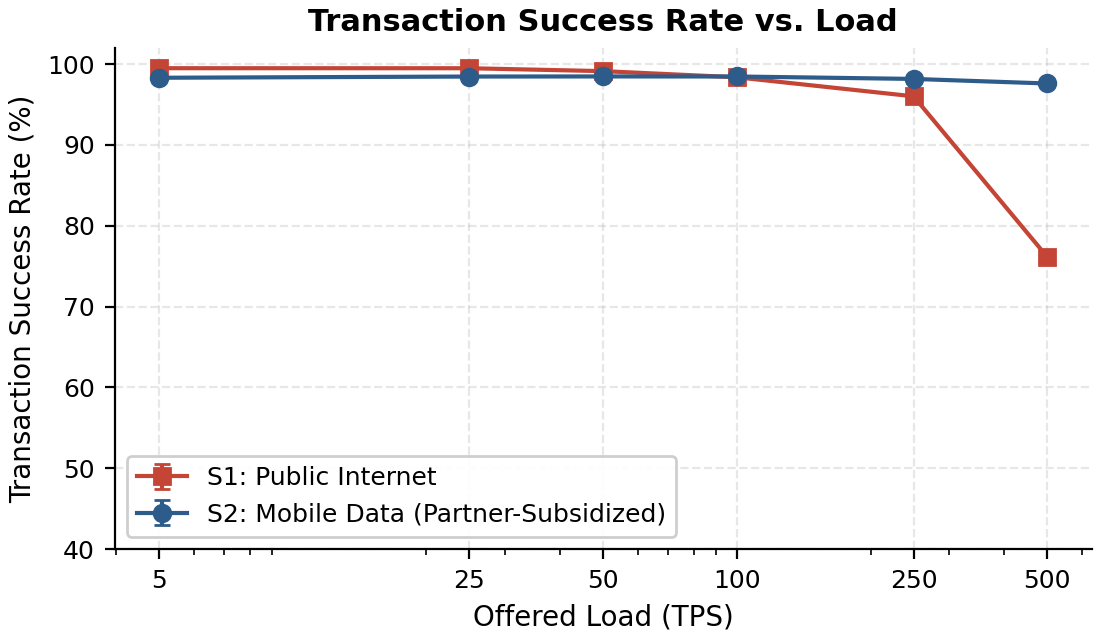
\includegraphics[width=\columnwidth]{fig6_success_rate.png}
\caption{Transaction success rate. S2 (Mobile Data) maintains approximately 97.6\% at 500 TPS, while S1 (public internet) degrades steeply under load.}
\label{fig:success}
\end{figure}

As shown in Fig.~\ref{fig:latency}, S2 demonstrates stable P95 latency near 672 ms at 500 TPS, with mild degradation driven by the load-dependent model. S1 experiences marked degradation, with P95 latency reaching approximately 14.5 s at 500 TPS, with the majority of failed transactions exceeding the 15 s E2E timeout.

\begin{figure}[t]
\centering
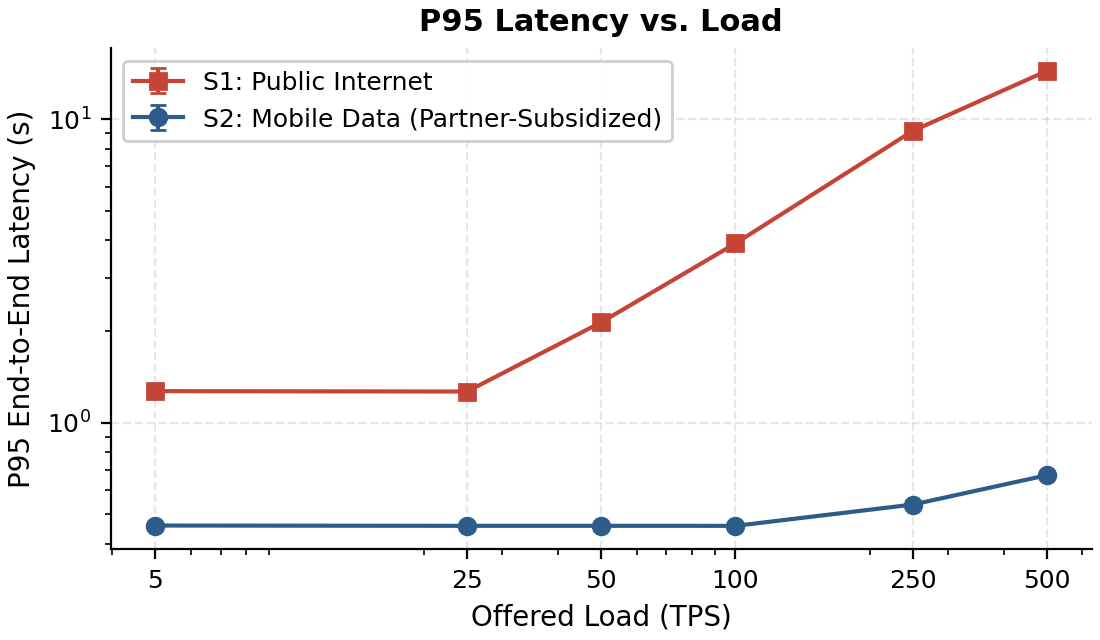
\includegraphics[width=\columnwidth]{fig7_p95_latency.png}
\caption{P95 end-to-end latency. S2 remains stable near 672 ms at 500 TPS; S1 inflates under load-dependent degradation.}
\label{fig:latency}
\end{figure}

According to internal evaluations of the Atheer Switch, the overhead was less than 20 ms. In all S1 failures, the switch was not the bottleneck; failures were overwhelmingly due to E2E timeouts caused by load-dependent latency degradation exceeding the 15 s timeout, with minimal contribution from packet loss. Table~\ref{tab:results} summarizes E2E performance across all load levels, while Table~\ref{tab:failures} provides the failure category breakdown at 500 TPS.

\begin{table}[t]
\caption{E2E Performance Summary (mean $\pm$ 95\% CI, $N=10$)}
\label{tab:results}
\centering
\footnotesize
\begin{tabular}{@{}ccccc@{}}
\toprule
\textbf{TPS} & \textbf{S1 Succ.\%} & \textbf{S2 Succ.\%} & \textbf{S1 P95 (s)} & \textbf{S2 P95 (s)} \\
\midrule
5   & 99.50$\pm$0.14 & 98.32$\pm$0.15 & 1.272$\pm$0.005 & 0.459$\pm$0.003 \\
25  & 99.50$\pm$0.06 & 98.47$\pm$0.05 & 1.268$\pm$0.003 & 0.458$\pm$0.001 \\
50  & 99.14$\pm$0.04 & 98.48$\pm$0.05 & 2.144$\pm$0.005 & 0.458$\pm$0.001 \\
100 & 98.38$\pm$0.03 & 98.48$\pm$0.04 & 3.902$\pm$0.011 & 0.458$\pm$0.001 \\
250 & 96.02$\pm$0.05 & 98.17$\pm$0.03 & 9.164$\pm$0.011 & 0.538$\pm$0.001 \\
500 & 76.15$\pm$0.05 & 97.61$\pm$0.02 & 14.451$\pm$0.004 & 0.672$\pm$0.000 \\
\bottomrule
\end{tabular}
\end{table}

\begin{table}[t]
\caption{Failure Breakdown at 500 TPS ($N=10$, summed counts)}
\label{tab:failures}
\centering
\footnotesize
\begin{tabular}{@{}lcccc@{}}
\toprule
\textbf{Scenario} & \textbf{Succ.\%} & \textbf{Uplink} & \textbf{Downlink} & \textbf{E2E TO} \\
\midrule
S1: Public Internet & 76.15\% & 0 & 134{,}452 & 280{,}129 \\
S2: Mobile Data & 97.61\% & 0 & 42{,}952 & 0 \\
\bottomrule
\end{tabular}
\end{table}

\subsection{Reproducibility and Data Availability}

In keeping with scientific transparency and DSR protocols, the complete source code for the DES (built with SimPy/Python) and the testing network scenarios of the four-layer Atheer architecture have been made open-source as a public research artifact \cite{mutawakel2024}. The repository includes simulation scripts, config files, deterministic seeds, results, and execution instructions.

% =================================================================
\section{Economic Analysis and Sustainability Model}
\label{sec:economic}
% =================================================================

Beyond technical validation, Atheer must address broader contextual factors to ensure the viability of its business model. This section analyzes how Atheer's architectural framework mitigates the most pertinent obstacles to financial service adoption, with a focus on the cost-optimized Mobile Data Routing model.

\subsection{Cost Model: Payload, Data, and Revenue}

The key economic insight of the revised architecture is that a tightly optimized 180-byte payload makes mobile data routing economically sustainable for the partner wallet. We formalize this via the following cost model.

\textbf{Daily Data Cost:} Let $N_{\mathrm{txn}}$ be the number of daily transactions, $P_{\mathrm{size}} = 180$ bytes the payload size, and $P_{\mathrm{data}}$ the mobile data price per megabyte. The daily data cost is:

\begin{equation}
C_{\mathrm{daily}} = \frac{N_{\mathrm{txn}} \cdot P_{\mathrm{size}}}{1{,}048{,}576} \cdot P_{\mathrm{data}}
\label{eq:cost}
\end{equation}

\textbf{MDR Revenue:} Let $A_{\mathrm{avg}}$ be the average transaction amount in USD and $r_{\mathrm{MDR}}$ the Merchant Discount Rate (typically 1--1.5\% in emerging markets). The daily MDR revenue is:

\begin{equation}
R_{\mathrm{daily}} = N_{\mathrm{txn}} \cdot A_{\mathrm{avg}} \cdot r_{\mathrm{MDR}}
\label{eq:revenue}
\end{equation}

\textbf{Cost Ratio:} The percentage of MDR revenue consumed by data cost is:

\begin{equation}
\rho = \frac{C_{\mathrm{daily}}}{R_{\mathrm{daily}}} \times 100\%
\label{eq:ratio}
\end{equation}

\subsection{Numerical Example}

Using realistic parameters for the Yemeni market:

\begin{itemize}
\item $N_{\mathrm{txn}} = 100{,}000$ daily transactions (nationwide partner wallet)
\item $P_{\mathrm{size}} = 180$ bytes
\item $P_{\mathrm{data}} = \$1.00$ per MB (Cable.co.uk upper bound for Yemen)
\item $A_{\mathrm{avg}} = \$5$ (typical micro-transaction)
\item $r_{\mathrm{MDR}} = 1\%$
\end{itemize}

\begin{equation*}
C_{\mathrm{daily}} = \frac{100{,}000 \times 180}{1{,}048{,}576} \cdot \$1.00 \approx \$17.17
\end{equation*}
\begin{equation*}
R_{\mathrm{daily}} = 100{,}000 \cdot \$5 \cdot 0.01 = \$5{,}000
\end{equation*}
\begin{equation*}
\rho = \frac{17.17}{5{,}000} \times 100\% \approx 0.34\%
\end{equation*}

The data cost consumes approximately \textbf{0.34\%} of MDR revenue, well below the 1\% threshold that would threaten economic sustainability. Figure~\ref{fig:cost} shows the sensitivity of this ratio across different data prices and transaction volumes.

\begin{figure}[t]
\centering
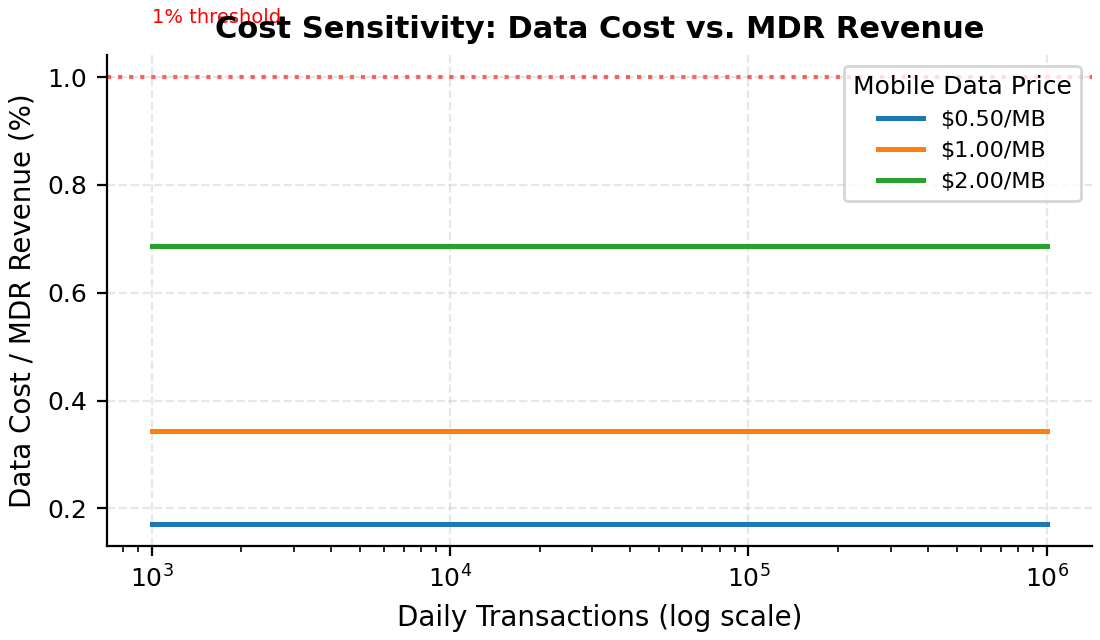
\includegraphics[width=\columnwidth]{fig8_cost_model.png}
\caption{Cost sensitivity: data cost as a percentage of MDR revenue, across mobile data prices and daily transaction volumes.}
\label{fig:cost}
\end{figure}

\subsection{Alleviating Barriers to Entry for Merchants}

\textbf{No Capital Expenditure:} A standard POS terminal costs between \$200 and \$600 per unit \cite{brandpos2024}. Atheer's SoftPOS uses the merchant's smartphone as the payment terminal, resulting in \$0 hardware cost. Combined with other factors, this enables a 60--80\% reduction in total cost of ownership for local businesses \cite{powertranz2024}.

\textbf{No Charge for Data:} The partner wallet absorbs the merchant's data cost through the B2B model described in Section~IV-C. The merchant pays nothing for data, even if their personal mobile data plan is exhausted.

\subsection{Value for Institutions}

\textbf{Banks:} Digital banking eliminates the ``cost of cash,'' improving cost-to-income ratios through reduced cash logistics \cite{ihl2024}. Banks also gain access to informal economy sales data, enabling better microfinance risk models \cite{banquedefrance2023}.

\textbf{Partner Wallets:} The wallet offering partner-subsidized data earns MDR revenue on every transaction. As shown in Section~VIII-B, this revenue dwarfs the data cost. The wallet also differentiates its service in a competitive market.

\textbf{Telecom Operators:} Standard mobile data traffic increases, with predictable revenue from partner wallets. Unlike private APN deployments, no special infrastructure investment is required.

\subsection{Comparison with Existing Systems}

Table~\ref{tab:comparison} compares Atheer with existing payment systems in similar markets.

\begin{table*}[t]
\caption{Comparison with Existing Payment Systems}
\label{tab:comparison}
\centering
\footnotesize
\begin{tabular}{@{}p{2.5cm}p{2.5cm}p{2.5cm}p{3cm}p{2.5cm}@{}}
\toprule
\textbf{Feature} & \textbf{Atheer} & \textbf{M-Pesa} & \textbf{Alkuraimi} & \textbf{Kipaad} \\
\midrule
Offline Capable & Yes (NFC) & Partial (USSD) & Partial (USSD) & Yes (NFC) \\
Hardware Cost & \$0 (SoftPOS) & \$0 & \$0 & POS required \\
Transport & Mobile Data & USSD/SMS & USSD/SMS & NFC + SIM \\
Multi-Provider & Yes & No (Safaricom) & No (single bank) & No \\
Payload Size & 180 bytes & N/A & N/A & N/A \\
Cost Model & Partner-subsidized & User-pays & User-pays & User-pays \\
\bottomrule
\end{tabular}
\end{table*}

\subsection{Ethical Disclaimer}

This economic analysis assumes a willing partner wallet operating under a documented B2B agreement. No specific Yemeni wallet is named as the partner; the model is presented as a general framework. The cost figures are derived from publicly available pricing data and do not require disclosure of any operator's proprietary commercial terms.

% =================================================================
\section{Conclusion}
% =================================================================

With regard to sustainable economic development goals, the Atheer system is one of the innovative FinTech solutions specifically developed for fragile and underdeveloped economies. We have shown that integrated NFC-based Host Card Emulation (HCE) combined with cost-optimized mobile data routing creates practical and dependable systems, achieving 97.6\% reliability at 500 TPS under simulated stress conditions. The 180-byte payload optimization enables a partner-subsidized billing model where data cost remains below 0.34\% of MDR revenue, making the architecture economically sustainable for nationwide rollout.

This system addresses three important areas that respond to current technical and regulatory challenges:

\begin{itemize}
\item \textbf{Reliability and scalability:} The mobile-data pathway has shown 97.6\% success at 500 TPS, providing a reliable alternative to public-internet-based systems without requiring special APN agreements with operators.

\item \textbf{Protection and confidentiality:} The system integrates a Biometric Cryptogram and Zero-Trust model to ensure data integrity while addressing spoofing and data fraud through information security best practices.

\item \textbf{Economic impact and financial inclusion:} Through zero-CapEx SoftPOS innovation and partner-subsidized data connectivity, the system offers considerable socio-economic advantages by expanding digital service accessibility to marginalized populations and digitizing the shadow economy. Atheer is both a technical proposal and an actionable blueprint that bridges theory to practice for e-wallet services and banks in conflict-affected areas.
\end{itemize}

% =================================================================
\section{Future Work}
% =================================================================

While we pursue this applied research, our short-term objectives focus on expanding cross-sector collaborations to develop further pilot projects.

\textbf{Case Study and Field Pilot:} We plan to conduct field tests involving cross-university, partner wallet, and public-private partnership collaborations. This will transform our framework into a live case study, allowing us to evaluate its direct and indirect impacts on business operations and financial inclusion.

\textbf{Governance and Regulatory Frameworks:} We will establish partnerships with banking institutions and regulators to create customizable proposals for the adoption and assessment of offline authorization frameworks, balancing data governance and anti-money laundering (AML) requirements.

\textbf{Formal Security Verification:} The security attributes established in this paper will undergo formal security verification using the Tamarin prover \cite{meier2013}, yielding machine-verified proofs of replay resistance and authentication correctness under the Dolev-Yao threat model. This will move the security claims from architecture-based arguments to formal verification.

% =================================================================
% References
% =================================================================
\begin{thebibliography}{35}

\bibitem{datareportal2024}
DataReportal, ``Digital 2024: Yemen,'' Kepios, 2024. [Online]. Available: \url{https://datareportal.com/reports/digital-2024-yemen}

\bibitem{ookla2024}
Ookla, ``Speedtest Global Index: Yemen,'' Ookla, 2024. [Online]. Available: \url{https://www.speedtest.net/global-index}

\bibitem{alhashedi2024}
A.~Al-Hashedi, N.~Almekhlafi, M.~T.~B.~Othman, and A.~Ghallab, ``An integrated theoretical model for cloud computing adoption in universities of Yemen,'' in \emph{Proc. 1st Int. Conf. Emerging Technol. Dependable Internet of Things (ICETI)}, Sana'a, Yemen, 2024, pp.~1--7.

\bibitem{almekhlafi2018}
N.~A.~Almekhlafi, ``Cloud computing awareness among practitioners in Yemeni universities,'' \emph{J. Sci. Technol.}, vol.~17, no.~2, pp.~46--55, 2018.

\bibitem{isoc2024}
Internet Society, ``Internet Resilience Index: Yemen,'' ISOC Pulse, 2024. [Online]. Available: \url{https://pulse.internetsociety.org/country/yemen}

\bibitem{gsma2023}
GSMA, ``The State of Mobile Internet Connectivity Report 2023,'' GSMA, London, U.K., 2023. [Online]. Available: \url{https://www.gsma.com/r/somic/}

\bibitem{imf2022}
International Monetary Fund, ``Fintech in the Middle East and Central Asia,'' IMF, Washington, DC, USA, IMF Policy Paper No.~2022/004, 2022.

\bibitem{worldbank2023}
World Bank, ``Yemen Digital Economy Assessment,'' World Bank Group, Washington, DC, USA, 2023. [Online]. Available: \url{https://documents.worldbank.org/}

\bibitem{brandpos2024}
BrandPOS, ``SoftPOS vs Traditional POS: A Complete Comparison,'' BrandPOS, 2024. [Online]. Available: \url{https://brandpos.com/blog/softpos-vs-traditional-pos/}

\bibitem{kemper2022}
G.~Kemper and L.~M.~Wulff, ``SoftPOS: The transformation of consumer devices into payment terminals,'' \emph{J. Payments Strategy Syst.}, vol.~16, no.~3, pp.~246--259, 2022.

\bibitem{ahamad2022}
S.~S.~Ahamad, ``A novel NFC-based secure protocol for merchant transactions,'' \emph{IEEE Access}, vol.~10, pp.~1905--1920, 2022.

\bibitem{oladapo2024}
O.~Oladapo \emph{et al.}, ``A review of tokenization and Host Card Emulation (HCE) in mobile payments,'' \emph{J. Cybersecurity Priv.}, vol.~4, no.~1, pp.~1--15, 2024.

\bibitem{gbadebo2024}
A.~Gbadebo, ``Short-lived distributed ledger technology for offline payments in emerging markets,'' \emph{African J. Inf. Syst.}, vol.~16, no.~1, pp.~1--20, 2024.

\bibitem{juniper2024}
Juniper Research, ``Global Soft POS Growth: Market Trends \& Forecasts 2024--2028,'' Juniper Research, Hampshire, U.K., 2024. [Online]. Available: \url{https://www.juniperresearch.com/}

\bibitem{hancke2010}
G.~P.~Hancke, ``Security challenges for RFID,'' in \emph{Proc. IEEE Int. Conf. RFID}, Orlando, FL, USA, 2010, pp.~253--260.

\bibitem{hevner2004}
A.~R.~Hevner, S.~T.~March, J.~Park, and S.~Ram, ``Design science in information systems research,'' \emph{MIS Quart.}, vol.~28, no.~1, pp.~75--105, Mar.~2004.

\bibitem{peffers2007}
K.~Peffers, T.~Tuunanen, M.~A.~Rothenberger, and S.~Chatterjee, ``A design science research methodology for information systems research,'' \emph{J. Manage. Inf. Syst.}, vol.~24, no.~3, pp.~45--77, 2007.

\bibitem{pci2023}
PCI Security Standards Council, ``PCI Contactless Payments Standard v1.0,'' PCI SSC, Wakefield, MA, USA, 2023. [Online]. Available: \url{https://www.pcisecuritystandards.org/}

\bibitem{dinh2021}
N.~T.~Dinh, Y.~Kim, and H.~Kim, ``A lightweight NFC-based mobile payment protocol for Internet of Things,'' \emph{IEEE Internet Things J.}, vol.~8, no.~14, pp.~11364--11373, 2021.

\bibitem{emvco2023}
EMVCo, ``EMV Contactless Specifications for Payment Systems,'' EMVCo, Geneva, Switzerland, Ver.~3.2, 2023. [Online]. Available: \url{https://www.emvco.com/}

\bibitem{rfc8446}
E.~Rescorla, ``The Transport Layer Security (TLS) Protocol Version 1.3,'' RFC 8446, IETF, Aug.~2018. [Online]. Available: \url{https://www.rfc-editor.org/rfc/rfc8446}

\bibitem{powertranz2024}
Powertranz, ``The Economics of SoftPOS,'' Powertranz, 2024. [Online]. Available: \url{https://powertranz.com/blog/economics-of-softpos/}

\bibitem{ihl2024}
IHL Group, ``Retail Cash Handling Costs and Shrinkage Report,'' IHL Group, Franklin, TN, USA, 2024.

\bibitem{banquedefrance2023}
Banque de France, ``Services in the Informal Sector,'' Banque de France, Paris, France, Econ. Bull., 2023.

\bibitem{meier2013}
S.~Meier, B.~Schmidt, C.~Cremers, and D.~Basin, ``The TAMARIN prover for the symbolic analysis of security protocols,'' in \emph{Proc. Int. Conf. Comput. Aided Verification (CAV)}, Springer, 2013, pp.~696--701.

\bibitem{mutawakel2024}
A.~Al-Mutawakel, ``Atheer Simulation Evaluation Artifact,'' GitHub Repository, 2024. [Online]. Available: \url{https://github.com/mutawakel-hub/atheer-research-artifacts}

\bibitem{itu2024}
International Telecommunication Union, ``ICT Price Baskets 2024,'' ITU, Geneva, Switzerland, 2024. [Online]. Available: \url{https://www.itu.int/en/ITU-D/Statistics/Pages/IPB/default.aspx}

\bibitem{cable2024}
Cable.co.uk, ``Worldwide Mobile Data Pricing 2024,'' Cable.co.uk, 2024. [Online]. Available: \url{https://www.cable.co.uk/mobiles/worldwide-data-pricing/}

\bibitem{roland2013}
M.~Roland, J.~Langer, and F.~Scharf, ``Applying relay attacks to Google Wallet,'' in \emph{Proc. Near Field Commun. (NFC)}, Zurich, Switzerland, 2013, pp.~1--6.

\end{thebibliography}

\end{document}
